%Corps du document :
%\setlength{\parindent}{1cm}    

\section{Conception détaillée}

Attachons nous maintenant à la conception détaille de notre application. Il s'agit
d'identifier et de spécifier les composants nécessaires pour automatiser tout ou
partie des outils à utiliser dans le cadre des cas d'utilisation identifiés.

Commençant par spécifier l'enchaînement des fenêtres grâce à un diagramme.

\subsection{Diagramme d'enchaînement des fenêtres}

\begin {center}
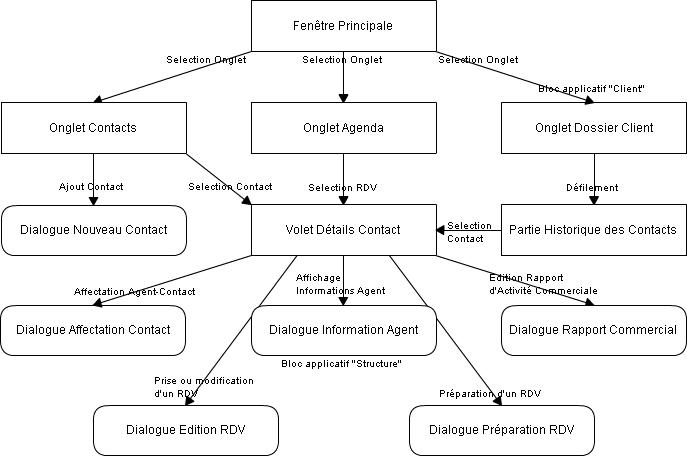
\includegraphics[width=\textwidth]{diagramme-edf.png}
\end {center}

\paragraph{Description}

L'Interface Homme-Machine (IHM) sera composée de trois onglets
principaux :

\begin{itemize}
\item \textbf{L'onglet Contacts} : Il présente la liste des Contacts prévus et affectés.
\item \textbf{L'onglet Agenda} : Il permet de consulter la liste des RDV pris.
\item \textbf{L'onglet Clients} : Cet onglet permet d'accéder aux dossiers des clients de la banque.
\end{itemize}

On observera également le volet \textbf{Détails du Contact}. Il permet d'effectuer toutes les
opérations nécessaires sur un Contact (une liste de ces services métiers se trouve plus loin
dans ce compte rendu).

\subsection{Dessin des fenêtres de l'IHM}

Voici une première représentation graphique de l'IHM que nous contruirons :

TODO @quentez

\subsection{Services Métiers invoqués par l'IHM}

Cette IHM offre différents services métiers. En voici la liste :

\begin{itemize}
\item Ajout d'un nouveau Contact
\item Affectation / Réaffectation d'un Contact
\item Prise / Modification d'un Rendez-Vous de Contact
\item Préparation d'un Rendez-Vous de Contact
\item Edition d'un Rapport d'Activité Commerciale suite à un Contact 
\end{itemize}

\subsection{Spécification des Services Métier}

TODO @xsauvagnat

\subsection{Spécification des Services Objets Métier}

TODO @xsauvagnat